\section{Stochastic Deployment Simulator}

All values used in this paper come from \texttt{results/simulate\_battery\_benchmark.py}, which generates the machine-readable benchmark file \texttt{results/demo\_benchmark.json} and the episode-level trace file \texttt{results/episode\_metrics.csv}. The simulator is not a physics engine. Instead, it is a compact deployment model that captures the variables needed for the scheduling claim: latent shift severity, battery depletion, adaptation latency, falls, distance, and compute energy.

The benchmark spans two shift families, terrain shift and payload shift, under two battery regimes: a low-battery state at $25\%$ and a high-battery state at $80\%$. Each regime evaluates the four policies described above over $1024$ stochastic episodes. For every policy we record mission return, distance traveled, system cost of transport, falls per $100$m, number of adaptation invocations, and adaptation-compute energy in watt-hours.

The simulator is designed to test one qualitative crossover. Low-battery regimes should punish over-frequent adaptation once compute and latency become non-trivial. High-battery regimes may still reward aggressive adaptation, because the controller can afford to spend more battery to maintain robustness. We further include an adaptation-cost sweep and a low-battery ablation to show how the crossover depends on the explicit cost model and the battery signal.

\begin{figure}[t]
\centering
\centering
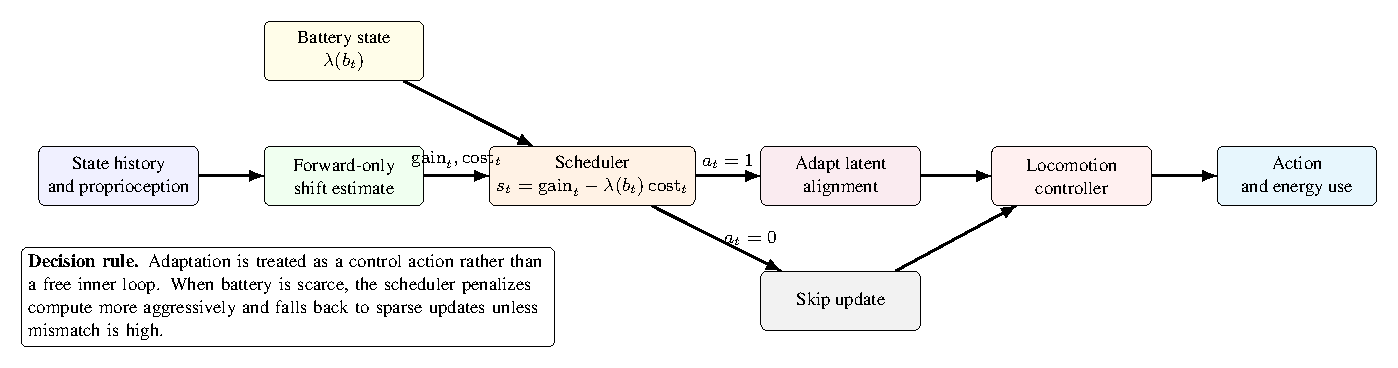
\includegraphics[width=0.98\linewidth]{../figure_assets/controller_schematic/controller_schematic.pdf}

\caption{Battery-gated forward-only adaptation pipeline. The scheduler treats adaptation as a control action, with the battery state modulating how aggressively compute is penalized.}
\label{fig:controller}
\end{figure}
